\documentclass[12pt,a4paper]{article}
%\documentclass[11pt,UTF8]{article}
%\usepackage{ctex}
\usepackage{tcolorbox}
\usepackage{graphicx}
\usepackage{geometry}
\usepackage{listings}
\usepackage{xcolor}
\usepackage{mathtools}
\usepackage{framed} 
\usepackage{amsfonts}
\usepackage{algpseudocode} 
\usepackage{algorithm}
\usepackage{ulem}
\usepackage{tikz}
\usepackage{amssymb}

\renewcommand{\algorithmicrequire}{ \textbf{Input:}} %Use Input in the format of Algorithm
\renewcommand{\algorithmicensure}{ \textbf{Output:}} %Use Output in the format of Algorithm
\definecolor{codegreen}{rgb}{0,0.6,0}
\definecolor{codegray}{rgb}{0.5,0.5,0.5}
\definecolor{codepurple}{rgb}{0.58,0,0.82}
\definecolor{backcolour}{rgb}{0.95,0.95,0.92}

\usepackage{tikz}
\usepackage{tikz-qtree}

\begin{document}
\noindent

%========================================================================
\noindent\framebox[\linewidth]{\shortstack[c]{
\Large{\textbf{Homework 1}}\vspace{1mm}\\
VE216 - Introduction to Signal and Systems, Qiao Heng, Spring 2021}}

\begin{center}

\footnotesize{\color{blue}$*$ Name:Han Yibei \quad Student ID: 519370910123 \quad Email: hyb\_2001@sjtu.edu.cn}
\end{center}

\section*{HW Notes:}
\begin{itemize}
    \item Problems where the number of points are followed by an exclamation are basic skill problems and will be graded without partial credit.
    \item \fbox{Box} your final answer. You will be graded on both the final answer and the steps leading to it. Correct intermediate steps will help earn partial credit.
    For full credit, \sout{cross out} any incorrect intermediate step.
    \item If you need to make any additional assumptions, state them clearly.
    \item Legible writing will help when it comes to partial credit.
    \item Simplify your result when possible.
\end{itemize}

\section*{Problems:}
\normalsize
\begin{tcolorbox}[colback = white]
1. Consider the sinusoidal signal illustrated below.\\
\begin{center}
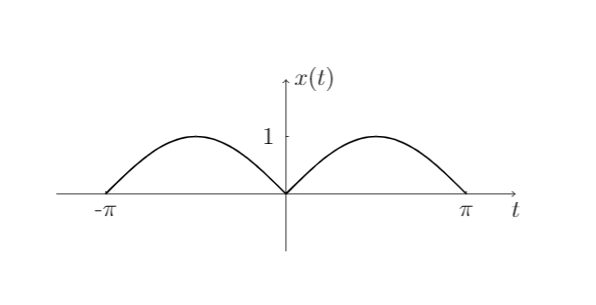
\includegraphics[scale=0.65]{problem1.png}\\
\end{center}
(a) [5!] Find the mathematical representation for this signal, where x(t) is 0 outside the interval $[-\pi,\pi]$;\\
(b) [5!] Carefully sketch and find a mathematical expression for the output signal of an integrator system, i.e., $y(t)=\int_{-\infty}^{t}x(\tau)d\tau$, where $x(t)$ is under the interval $[-\pi,\pi]$.
\end{tcolorbox}

\begin{tcolorbox}
\normalsize
\textcolor{blue}{Answer:\\
(a) \fbox{$x(t)=rect(\frac{t}{2\pi})\times |sin(x)|$}\\
(b)~$rect(\frac{t}{2\pi})=u(t+\pi)u(-ket-\pi)$\\
$$f(x)=u(t+\pi)u(t-\pi)|sin(x)|$$
$$y(t)=\int^t_{-\infty}x(\tau)d\tau=$$
for $t<-\pi$, $y(t)=0$\\
for $-\pi<t<0$, $x(t)=-sin(\tau)$, so \fbox{$y(t)=\int_{-\pi}^t-sin(\tau)=1+cos(t)$}\\
for $0<t<\pi$, $x(t)=sin(\tau)$, so \fbox{$y(t)=\int^t_0sin(\tau)=3-cos(t)$}\\
for $t>\pi$, $y(t)=4$
\begin{figure}[H]
    \centering
    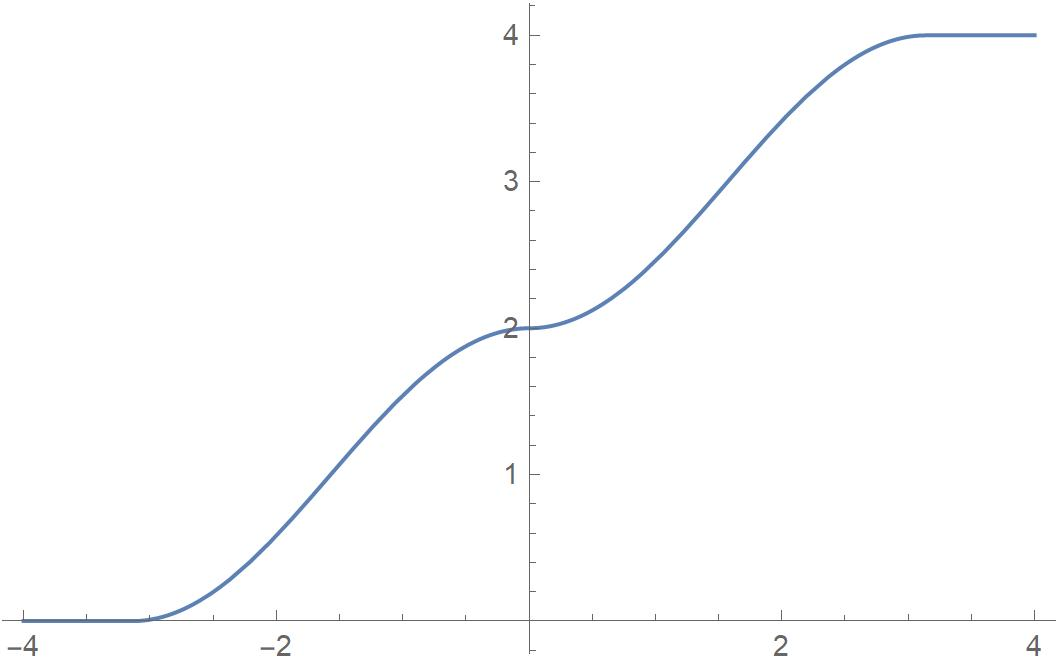
\includegraphics[width=8cm]{1b.jpg}
\end{figure}
}
\end{tcolorbox}

\begin{tcolorbox}[colback = white]
2. [10!] Calculate the average value, power and energy of signal f(n) =
$$\begin{cases} 
e^{-2t},  & t>0, \\
0, & \mbox{otherwise.}
\end{cases}$$
Is it an energy signal, power signal, or neither?
\end{tcolorbox}

\begin{tcolorbox}
\normalsize
\textcolor{blue}{Answer:
$$\text{Average: }A\triangleq\lim_{T\to\infty}\frac{1}{2T}\int^{T}_{-T}x(t)dt=\lim_{T\to\infty}\frac{1-e^{-2T}}{4T}=\fbox{0}$$
$$\text{Energy: }E\triangleq\int^\infty_{-\infty}|x(t)|^2dt=\int^\infty_0e^{-4t}dt=\fbox{$\frac{1}{4}$}$$
$$\text{Power Signal: }P\triangleq\lim_{T\to\infty}\frac{1}{2T}\int^{T}_{-T}|x(t)|^2dt=\lim_{T\to\infty}\frac{1-e^{-4T}}{8T}=\fbox{0}$$
It is an \fbox{energy signal}.
}
\end{tcolorbox}

\begin{tcolorbox}[colback = white]
3. Suppose $x_1(t)$ and $x_2(t)$ are two periodic signals with fundamental periods $T_1>0$ and $T_2>0$ respectively.\\
(a) [5!] Show that if $T_1/T_2$ is rational, then $x(t)=x_1(t)+x_2(t)$ is periodic.\\
(b) [5!] Show that if $T_1/T_2$ is rational, then $x(t)=x_1(t)x_2(t)$ is periodic and the least common multiple of $T_1$ and $T_2$ is a period of $x(t)$.\\
(c) [5!] Determine whether the following signals are periodic. If so, find a period. If not, specify the reason.
\begin{center}
$x_1(t)=\mbox{sin}(\pi t/3)\mbox{cos}(\pi t/7)+\mbox{sin}(\pi t/5)\mbox{sin}(\pi t/11)$\\
\end{center}
\begin{center}
$x_2(t)=\mbox{sin}(\sqrt{3}\pi t/3)+\mbox{sin}(\pi t/7)$\\
\end{center}
\end{tcolorbox}

\begin{tcolorbox}
\normalsize
\textcolor{blue}{Answer:\\
(a) Since $\frac{T_1}{T_2}$ is rational, there must exist certain $T_3=aT_1=bT_2$, while a and b are integers
$$x_1(t)=x_1(t+T_1)~ \forall t~~~~x_1(t)=x_1(t+T_1)~\forall t$$
$$\rightarrow x_1(t)+x_2(t)=x_1(t+T_3)+x_2(t+T_3)~\forall t$$
so $x_1+x_2$ is periodic.\\
(b) Since $\frac{T_1}{T_2}$ is rational, there must exist certain $T_3=aT_1=bT_2$, while a and b are integers
$$x_1(t)=x_1(t+T_1)~ \forall t~~~~x_1(t)=x_1(t+T_1)~\forall t$$
$$\rightarrow x_1(t)\times x_2(t)=x_1(t+T_3)\times x_2(t+T_3)~\forall t$$
so $x_1\times x_2$ is periodic.\\
Also, with the condition that $aT_1=bT_2$, T must be the least common multiple of $T_1$ and $T_2$
(c) As a, b have determined, 1 is periodic and the smallest period is lcm($T_1$, $T_2$, $T_3$, $T_4$)=lcm(6, 14, 10, 22)=\fbox{2310}.\\
2 is \fbox{not periodic} since the divide product of period of $sin(\sqrt{3}\pi t/3)$ and $sin\pi t/7$ is not rational
}
\end{tcolorbox}

\begin{tcolorbox}[colback = white]
4. [20!]Indicate whether the following systems are Memoryless, Time Invariant, Linear, Causal, Stable. Justify your answers.\\
(a) $y(t)=x(t-3)+x(3-t)$\\
(b) $y(t)=\cos{(4x(t))}$\\
(c) $y(t)=\int_{-\infty}^{t/3}x(\tau)d\tau$
\end{tcolorbox}

\begin{tcolorbox}
\normalsize
\textcolor{blue}{Answer:\\
(a) \fbox{Not memoryless, not time invariant, linear, not causal, stable}\\
\textbf{Memoryless:} The system is NOT memoryless because the output at time t depends on input values at times other than t\\ \\
\textbf{Time invariance:} This system is time invariant. We let y(t) be the output corresponding to the input x(t) and $x_a(t)=x(t-a)$. Then
\begin{equation*}
    \begin{aligned}
        y_a(t)&=x_a(t-3)+x_a(3-t)\\
        &=x(t-a-3)+x(3-t-a)\\
        &\neq x((t-a)-3)+x(3-(t-a))=y(t-t_0)
    \end{aligned}
\end{equation*}
\textbf{Linearity:} The system is linear because
\begin{equation*}    
    \begin{aligned}
        y_1(t)=&x_1(t-3)+x_1(3-t)\\
        y_2(t)=&x_2(t-3)+x_2(3-t)\text{ and}\\
        x(t)=&\alpha x_1(t)+\beta x_2(t)
    \end{aligned}
\end{equation*}
then the output y(t) corresponding to the input x(t) is
\begin{equation*}
    \begin{aligned}
        y(t)&=x(t-3)+x(3-t)\\
        &=(\alpha x_1+\beta x_2)(t-3)+(\alpha x_1+\beta x_2)(3-t)\\
        &=\alpha(x_1(t-3)+x_1(3-t))+\beta(x_2(t-3)+x_2(3-t))\\
        &=\alpha y_1(t)+\beta y_2(t)
    \end{aligned}
\end{equation*}
\textbf{Causality:} The system is not causal, for example: y(0)=y(-3)+y(3), so it depends on future input\\
\textbf{Stability:} $y(t)=x(t-3)+x(3-t)<x_{Max}+x_{Max}=2x_{Max}$, let $y_{Max}=2x_{Max}+1$, $|y(t)|<y_{Max}$
}
\end{tcolorbox}

\begin{tcolorbox}
    \normalsize
    \textcolor{blue}{Answer:\\
    (b) \fbox{Memoryless, time invariant, not linear, causal, stable}\\
    \textbf{Memoryless:} The system is memoryless because the output at time t depends on input values at time t\\ \\
    \textbf{Time invariance:} This system is time invariant. We let y(t) be the output corresponding to the input x(t) and $x_a(t)=x(t-a)$, let $x(t)=\delta(t)$. Then
    \begin{equation*}
        \begin{aligned}
            y_a(t)&=cos(4x_a(t))\\
            &=cos(4x(t-a))\\
            &=y(t-a)
        \end{aligned}
    \end{equation*}
    \textbf{Linearity:} The system is not linear because
    \begin{equation*}    
        \begin{aligned}
            y_1(t)=&cos(4x_1(t))\\
            y_2(t)=&cos(4x_2(t))\text{ and}\\
            x(t)=&\alpha x_1(t)+\beta x_2(t)
        \end{aligned}
    \end{equation*}
    then the output y(t) corresponding to the input x(t) is
    \begin{equation*}
        \begin{aligned}
            y(t)&=cos(4x(t))\\
            &=cos(4()\alpha x_1(t)+\beta x_2(t)))\\
            &\neq \alpha y_1(t)+\beta y_2(t)
        \end{aligned}
    \end{equation*}
    \textbf{Causality:} The system is causal because the output only depend on the current t\\
    \textbf{Stability:} $|y(t)|<1$, the output is bounded
    }
    \end{tcolorbox}

    \begin{tcolorbox}
        \normalsize
        \textcolor{blue}{Answer:\\
        (c) \fbox{Not memoryless, not time invariant, linear, not causal, not stable}\\
        \textbf{Memoryless:} The system depends on t in past, future or current depends on $x(\tau)$. So we cannot tell whether it is memoryless or not.\\ \\
        \textbf{Time invariance:} This system is NOT time invariant. We let y(t) be the output corresponding to the input x(t) and $x_a(t)=x(t-a)$. Then
        \begin{equation*}
            \begin{aligned}
                y_a(t)&=\int^{t/3}_{-\infty}x(\tau-\tau_0)d\tau\\
                &=\int^{t/3-\tau_0}_{-\infty}x(\tau)d\tau\\
                &\neq\int^{(t-\tau_0)/3}_{-\infty}x(\tau)d\tau=y(t-a)Legible
            \end{aligned}
        \end{equation*}
        \textbf{Linearity:} The system is linear because
        \begin{equation*}    
            \begin{aligned}
                y_1(t)=&\int^{t/3}_{-\infty}x_1(\tau)d\tau\\
                y_2(t)=&x\int^{t/3}_{-\infty}x_2(\tau)d\tau\text{ and}\\
                x(t)=&\alpha x_1(t)+\beta x_2(t)
            \end{aligned}
        \end{equation*}
        then the output y(t) corresponding to the input x(t) is
        \begin{equation*}
            \begin{aligned}
                y(t)&=\int^{t/3}_{-\infty}(\alpha x_1+\beta x_2)(\tau)d\tau\\
                &=\alpha y_1(t)+\beta y_2(t)
            \end{aligned}
        \end{equation*}
        \textbf{Causality:} The system depends on t in past, future or current depends on $x(\tau)$. So we cannot tell whether it is causal or not.\\
        \textbf{Stability:} $y(t)=x(t-3)+x(3-t)<x_{Max}+x_{Max}=2x_{Max}$, let $y_{Max}=2x_{Max}+1$, $|y(t)|<y_{Max}$
        }
        \end{tcolorbox}    

\newpage
\begin{tcolorbox}[colback = white]
5. Consider the signal illustrated below.
\begin{center}
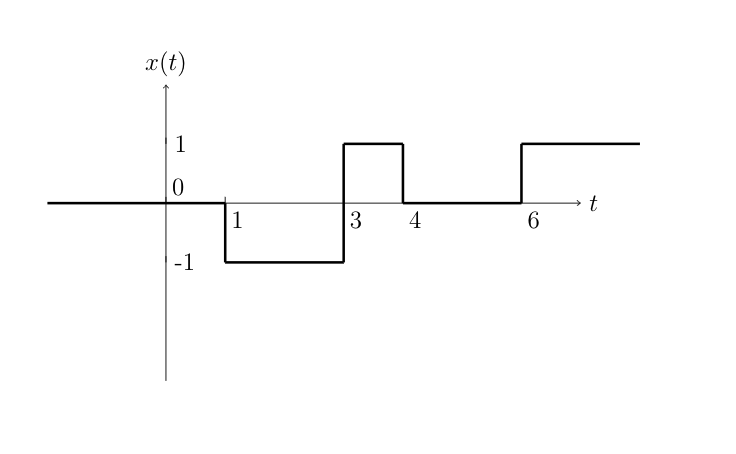
\includegraphics[scale=0.5]{problem5.png}
\end{center}
(a) [5!] Express the signal $x(t)$ using a sum of step functions.\\
(b) [5!] Find the derivative of the signal and carefully sketch it.
\end{tcolorbox}

\begin{tcolorbox}
\normalsize
\textcolor{blue}{Answer:\\
(a) \fbox{x(t)=-u(t-1)+2u(t-3)-u(t-4)+u(t-6)}\\
(b) \fbox{x'(t)=$-\delta(t-1)+2\delta(t-3)-\delta(t-4)+\delta(t-6)$}\\
\begin{figure}[H]
    \centering
    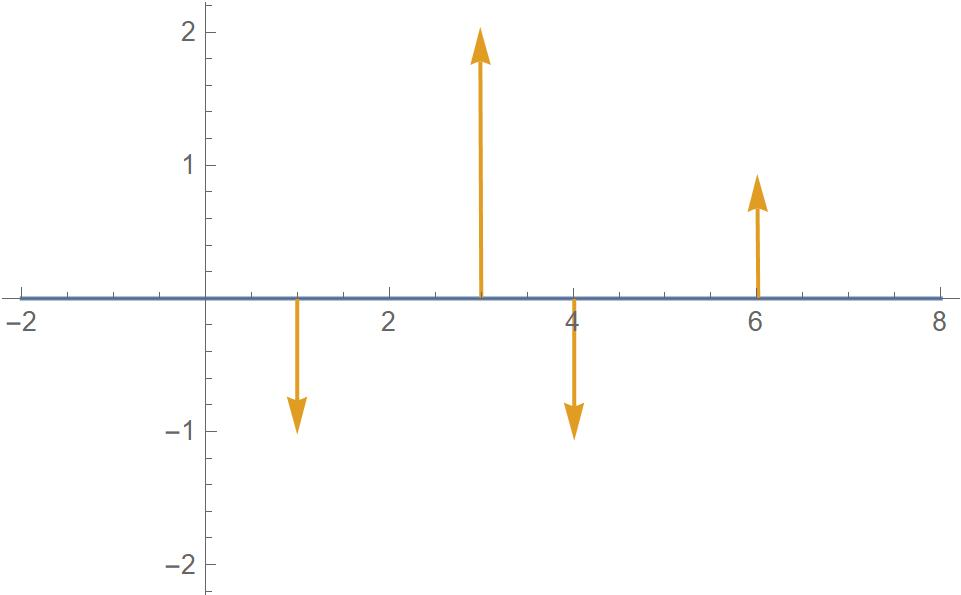
\includegraphics[width=8cm]{5b.jpg}
\end{figure}
}
\end{tcolorbox}

\begin{tcolorbox}[colback = white]
6. A system H has following input-output pairs. Answer the following question, and justify your answers\\
\begin{center}
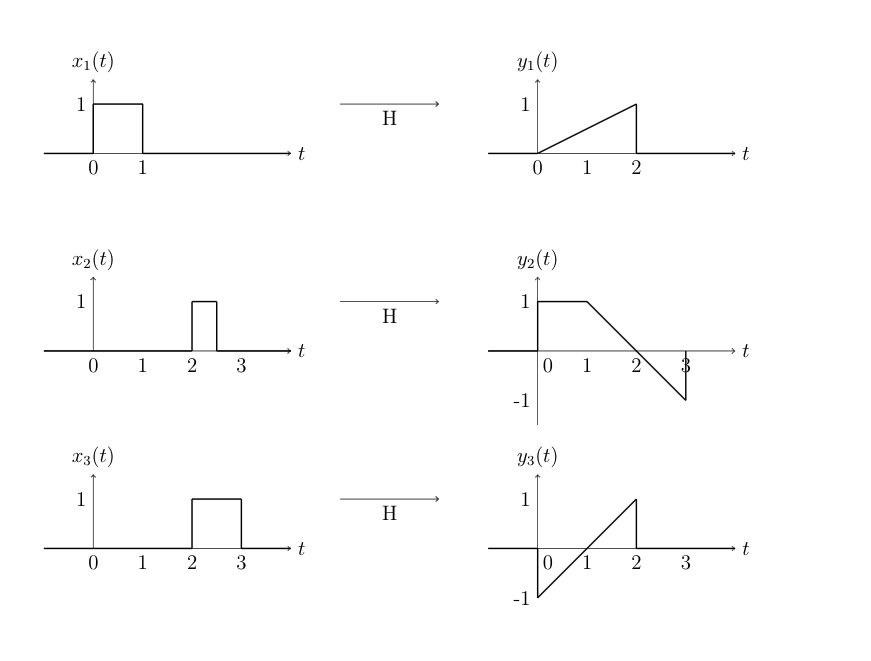
\includegraphics[scale=0.45]{problem6.png}
\end{center}
(a) [5!] Could this system be causal?\\
(b) [5!] Could this system be time invariant?
\end{tcolorbox}

\begin{tcolorbox}
\normalsize
\textcolor{blue}{Answer:\\
(a) No\\
In figure 2 and 3, the 0-2 both zero. But the output is not the same.\\
(b) No\\
In figure 1 and 3, the input change 2 unit, but the output did not only change 2 unit.
}
\end{tcolorbox}

\begin{tcolorbox}[colback = white]
7. Consider the signal $s(t)=(\frac{t-1}{2})^2rect(\frac{t-1}{2}$)\\
(a) [3!] Make a sketch of $s(t)$\\
(b) [7!] Evaluate $\int_{-\infty}^{\infty}s(t)x(t)dt$, where $x(t)=\delta(2t-1)+\delta(t-2)-\delta(3t-5)$\\
(You do not need to give the numeric value. It is OK to leave the expression with $s(t)$)
\end{tcolorbox}
\begin{tcolorbox}
\normalsize
\textcolor{blue}{Answer:\\
(a)
\begin{figure}[H]
    \centering
    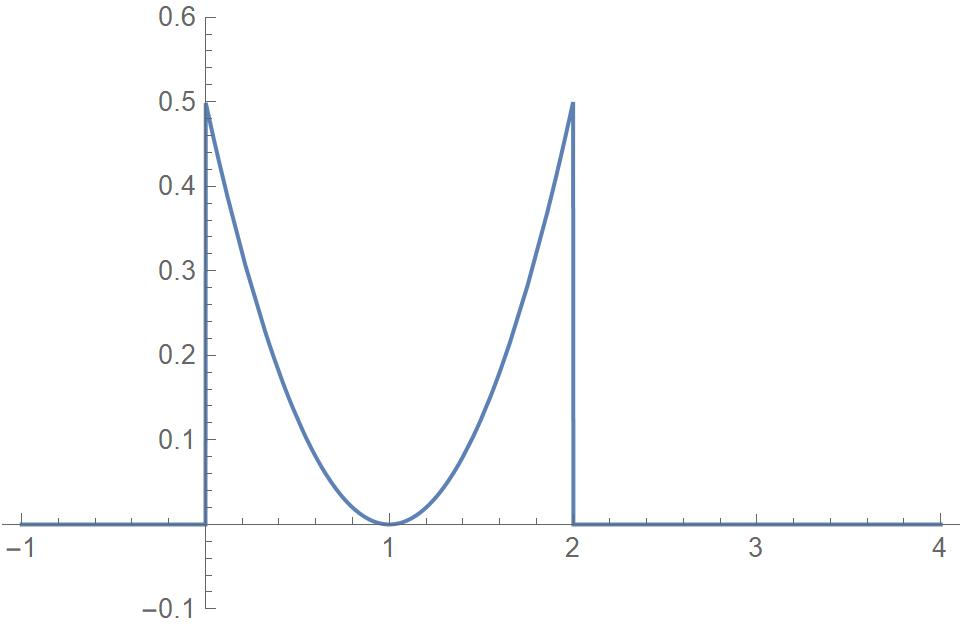
\includegraphics[width=8cm]{7a.jpg}
\end{figure}
(b) \fbox{$\frac{1}{2}$s($\frac{1}{2}$)+s(2)-$\frac{1}{3}$s($\frac{5}{3}$)}
}
\end{tcolorbox}

\begin{tcolorbox}[colback = white]
8. For $x(t)$ indicated in the following figure, sketch the following:\\
(a) [2!] $x(-t)$\\
(b) [3!] $x(t+2)$\\
(c) [5!] $x(2t+2)$\\
(d) [5!] $x(1-3t)$\\
\begin{center}
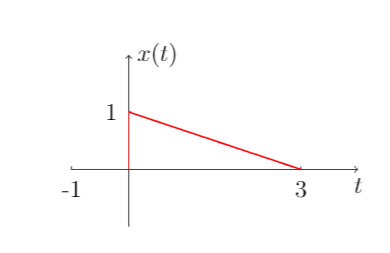
\includegraphics[scale=1]{problem8.png}
\end{center}
\end{tcolorbox}
\begin{tcolorbox}
\normalsize
\textcolor{blue}{Answer:\\
(a) x(-t)
\begin{figure}[H]
    \centering
    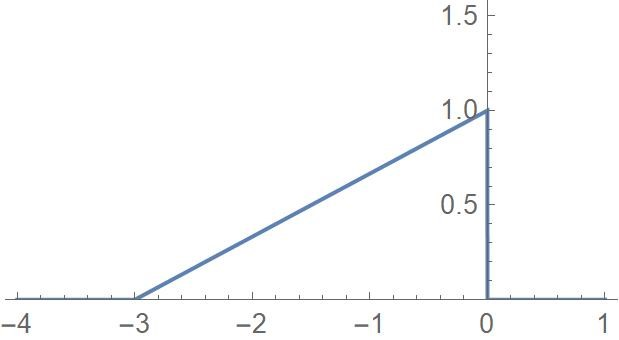
\includegraphics[width=6cm]{8a.jpg}
\end{figure}
(b) x(t+2)
\begin{figure}[H]
    \centering
    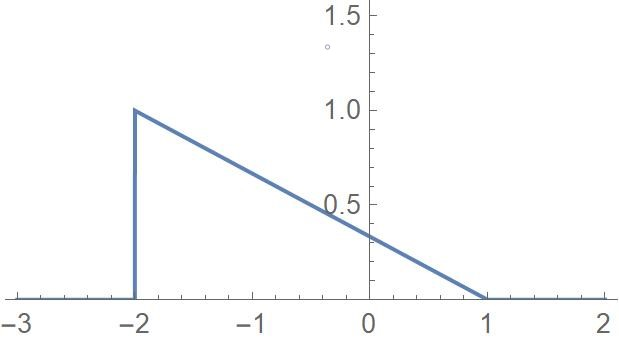
\includegraphics[width=6cm]{8b.jpg}
\end{figure}
(c) x(2t+2)
\begin{figure}[H]
    \centering
    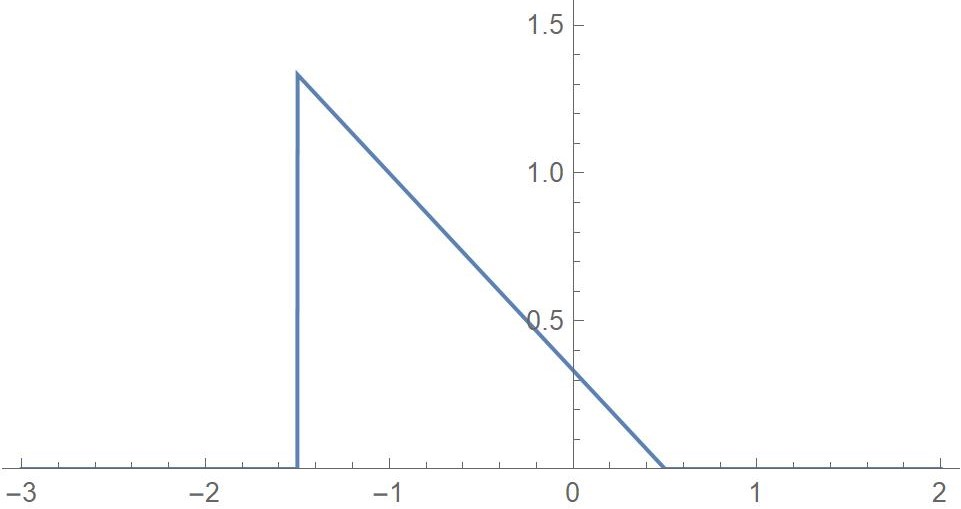
\includegraphics[width=6cm]{8c.jpg}
\end{figure}
(d) x(1-3t)
\begin{figure}[H]
    \centering
    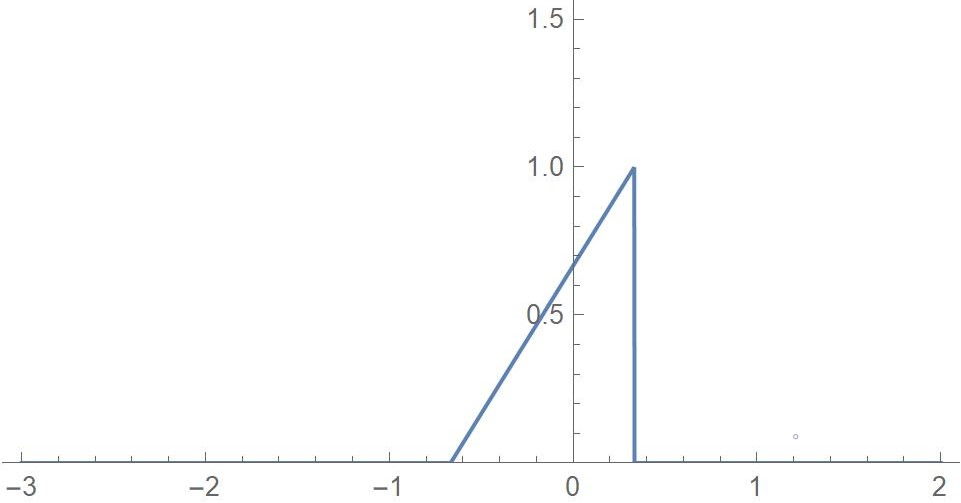
\includegraphics[width=6cm]{8d.jpg}
\end{figure}
}


\end{tcolorbox}

%========================================================================
\end{document}
